\documentclass[conference]{IEEEtran}
\usepackage{cite}
\usepackage{array}
\usepackage{graphicx}
\usepackage{float} %used to force figures in a position
\hyphenation{op-tical net-works semi-conduc-tor}

\begin{document}
\title{Building a Compilator on Java for a mini-C Programming Language}

\author{\IEEEauthorblockN{J. Agust\'{i}n Barrachina}
\IEEEauthorblockA{IEEE Student Member\\
\'{E}cole Polytechnique\\
Universit\'{e} Saclay-Paris}
\and
\IEEEauthorblockN{Phil\'{e}mon Poux}
\IEEEauthorblockA{\'{E}cole Polytechnique\\
	Universit\'{e} Saclay-Paris}}
\maketitle

\tableofcontents
\newpage

\begin{abstract}
In this project, a compilator was created to generate a x86-64 assembler code from a C fragment called mini-C.
This is a 100\% C-compatible fragment, in the sense that any Mini C program is also a C program. 
\end{abstract}

\IEEEpeerreviewmaketitle

\section{Introduction}
\textit{"Optimizing compilers are so difficult to get right that we dare say that no optimizing compiler is error-free! Thus, the most important objective in writing a compiler is that it is correct"}\cite{DRAGON_BOOK}

The reader is suppose to have some basic knowledge of C and for that reason almost no explanation regarding that language will be treated in this report. For further information about C language refer to \cite{LANGUAGE_C}.

Simply stated, a Compiler is a program that can read a code written in a specific programming language and translate it into an equivalent code of another language. A fairly good analogy can be made by a translator between two different languages like Spanish and French for example.

The objective of this project is to create a compiler for a fragment of C denominated \textit{Mini C}. Produce a reasonably effective code x86-64. \textit{Mini C} is a fragment of the language C which contains integers and pointers to structures. \textit{Mini C} is 100\% compatible with C in the sense that every \textit{Mini C} program is also a C program. This will enable to use a C compiler such us \textbf{gcc} to use as reference. 

\subsection{Structure of a Compiler}\label{sub_structure_of_a_compiler}

A compiler can be divided into two parts. The \textit{analysis} (front end) and the \textit{synthesis} (back end)

The \textit{analysis} brakes the source program into constituent pieces and imposes a grammatical structure of them in order to create a intermediate representation of the source program. During this part, syntactical formation and semantical unsound is checked. The analysis also collects information about the source program and stores it in a data structure called a \textit{symbol table} which will be used by the \textit{synthesis} part.

The \textit{synthesis} part makes use of the \textit{symbol table} and the intermediate representation constructed by the analysis part and creates the target program.

A more detailed diagram of the structure can be seen in figure \ref{fig_struct_of_compilator}. Where the last part (Code Generation) correspond to the \textit{synthesis} phase and the rest are all from the \textit{analysis} phase. The diagram is longer that the one displayed, having also a converser from the assembler to the machine language and from there to the executable code. But in this project, those stages are not treated.

\begin{figure}[H]
\centering
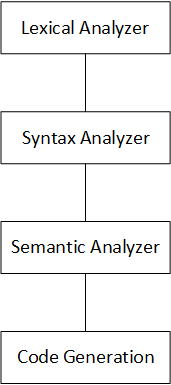
\includegraphics[width=3cm]{images/Diagram.png}
\caption{Structure of a Compiler}
\label{fig_struct_of_compilator}
\end{figure}

\section{Lexical Analyzer}
A lexical analyzer (\textit{Lexer}) is the first front-end step in compilers, matching keywords, comments, operators, etc, and generating a token stream for parsers called \textit{lexemes} consisting of a \textit{token name} and the \textit{attribute value}. 
The \textit{token name} is an abstract symbol that will be used during syntax analysis, while the \textit{attribute value} is an entry in the \textit{symbol table} (discussed on \ref{sub_structure_of_a_compiler}) which will be used during the semantic analysis and the code generation.

The Lexer reads input from the programming language to compile (mini c in our case) and matches it against regular expressions and runs a corresponding action if such an expression is matched.

To make the Lexer are going to use:
\begin{itemize}
	\item Regular Expressions: To describe the lexemes
	\item Finite Automata: To recognize the expressions
\end{itemize}
\subsection{Regular Expressions}
The concept of regular expression arose in the 1950's when the American mathematician Stephen Cole Kleene formalized the description of a regular language.

A regular expression is a sequence of characters that define a search pattern. In other words, there are a conjunction of letters and digits that follow a certain rule.

Let us define \textit{letter} as any letter in the Latin alphabet and \textit{digit} any number [0-9]. Then we can define rules as follow: 
\begin{equation}
0 | [1-9] (<digit>* | [])\label{reg_expr_example}
\end{equation}

Last equation \ref{reg_expr_example} is a declaration of a decimal digit. The "$|$" is a logic or, it means, either the digit is 0 or it will be another thing. If it is not only 0, the number cannot start by 0 in C syntax, so it must start with a digit different from 0, which is range from 1 to 9 (encoded as [0-9]). Secondly, this digit can be followed by either nothing (represented by: []) or by any digit for as many digits are they must be. The format $<$rule$>$* means the repetition of a rule for as many times as necessary, or no repetition at all.

% We could add another example here, for example a comment line or sth.
\subsection{Finite Automata}
A \textit{finite automata} is basically a binary graph which just say "yes" or "no" by means of a \textit{recognizer} to each possible string.

There are two different classes of automatas:
\begin{enumerate}
	\item \textit{Nondeterministic Finite Automata} (NFA)
	\item \textit{Deterministic Finite Automata} (DFA)
\end{enumerate}
The first class (NFA) have no restrictions on the labels of their edges. A symbol can label several edges out of the same state. The DFA on the other hand have for each state and symbol exactly one edge with that symbol leaving that state. 
%translate to english...

\subsection{Implementation}
%The corresponding action will be just to generate an abstract symbol (normally called "token name") that can be read by the next phase (Syntax Analyzer).

For the lexical analyzer, a flex library was used \cite{JFLEX}. A .flex file was created and then, by means of jflex, converted to the final java class.

Jflex lexers are based on a DFA automata. For more information about jflex library please refer to \cite{JFLEX_MANUAL}. 

\section{Syntax Analyzer} \label{sub_syntax_analyzer}

The syntax of a programming language describes the proper form of its programs.

The \textit{syntax analyzer} or \textit{parser} uses the first component of the \textit{lexemes}, the \textit{tokens}. The \textit{parser} creates some kind of tree representation that depicts the grammatical structure of the token stream called the \textit{syntax tree}. In this tree, each node represent an operation and the children of the node represent the arguments of that operation. 

\begin{figure}[H]
	\centering
	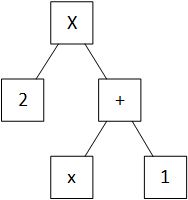
\includegraphics[width=3cm]{images/syntax_tree.png}
	\caption{Syntax Tree Example}
	\label{fig_syntax_tree_example}
\end{figure}

On figure \ref{fig_syntax_tree_example} an example of a tree representation can be seen. Many syntaxes can be the cause of that tree, for example, both \ref{(2*((x)+1))} and \ref{2*(x+1)} can be used to generate such tree.

\begin{equation}
2*(x+1)
\label{2*(x+1)}
\end{equation}

\begin{equation}
(2*((x)+1))
\label{(2*((x)+1))}
\end{equation}

\subsection{Implementation}

The Syntax Analyzer was done using CUP, a parser generator for java \cite{CUP}.

In that file, precedence where applied to each operator using the following table:
\begin{table}[H]
	\begin{center}
	\begin{tabular}{||c c||}
		\hline
		Operator & Associativity  \\ [0.5ex] 
		\hline\hline
		= & right \\ 
		\hline
		$|$$|$ & left  \\
		\hline
		\&\& & left  \\
		\hline
		== != & left  \\
		\hline
		$<$ $<$= $>$ $>$= & left \\ [1ex] 
		\hline
		+ - & left \\
		\hline
		* / & left \\
		\hline
		! -(negative) & right \\
		\hline
		-$>$ & left \\
		\hline
	\end{tabular}
	\end{center}
	\caption{Precedence} \label{tab_precedence}
\end{table}

The higher the operator is in the table, the last will it be applied. For example, the operator "=" will be applied after all the other operators have been applied. There is a very simple way to apply this table in the .cup file by simply writing the following command: precedence <associativity> <token name>. Where associativity is either left or right and the token name is the token from the \textit{lexem} created by the Lexer.

After the precedence, the following grammar was implemented (table \ref{tab_grammar}). The details on how to implement it where omitted. In order to see how to implement the following grammar in cup please refer to the user manual \cite{CUP_MANUAL}.

\begin{table}[H]
	\begin{center}
		\begin{tabular}{ | m{1.5cm} | m{6.5cm}| } 
			\hline
			$<$ file $>$ & $<$ decl $>$* EOF \\ 
			\hline
			$<$ decl $>$ & $<$ var $>$ $|$ $<$ type $>$ $|$ $<$ funct $>$ \\ 
			\hline
			$<$ var $>$ & int $<$ ident $>^{+},$ ; \newline 
						struct $<$ ident $>$ ( *$<$ ident $>^{+},$ ) ; \\ 
			\hline
			$<$ type $>$ & struct $<$ ident $>$ { $<$ var $>$* } ; \\
			\hline
			$<$ funct $>$ & int $<$ ident $>$ ( $<$ param $>^{*},$ ) $<$ bloc $>$ \newline 
							struct $<$ ident $>$ * $<$ ident $>$ ($<$ param $>^{*},$) $<$ bloc $>$ \\
			\hline
			$<$ param $>$ & int $<$ ident $>$ $|$ struct $<$ ident $>$ * $<$ ident $>$ \\
			\hline
			$<$ expr $>$ & 	$<$ integer $>$ \newline 
							$<$ ident $>$ \newline
							$<$ expr $>$ -$>$ $<$ ident $>$ \newline
							$<$ ident $>$ ( $<$ expr $>^{*},$ ) \newline 
							! $<$ expr $>$ $|$ -$<$ expr $>$ \newline
							$<$ expr $>$ $<$ op $>$ $<$ expr $>$ \newline
							sizeof ( struct $<$ ident $>$ ) \newline
							( $<$ expr $>$ )	\\
			\hline
			$<$ op $>$ & = $|$ == $|$ != $|$ + $|$ - $|$ * $|$ / $|$ \&\& $|$ $<$ $|$ $<$= $|$ $>$ $|$ $>$= $|$ $|$$|$ \\ 
			\hline
			$<$ instr $>$ & ; \newline
							$<$ expr $>$; \newline
							if ( $<$ expr $>$ ) $<$ instr $>$\newline
							if ( $<$ expr $>$ ) $<$ instr $>$ else $<$ instr $>$ \newline
							while ( $<$ expr $>$ ) $<$ instr $>$ \newline
							$<$ bloc $>$ \newline
							return $<$ expr $>$; \\				
			\hline
			$<$ instr $>$ & { $<$ var $>*$ $<$ instr $>*$  } \\
			\hline
		\end{tabular}
	\end{center}
	\caption{Grammar} \label{tab_grammar}
\end{table}

Where '$|$' is either one or the other is found. The '*' is as many as necessary (including none at all), while on the other hand, '+' means as many as necessary but at least one. If under any of those symbols there is a comma (',') it means there are comma indented.

Within a file, one will find a list of declarations. These declarations can be either a variable or structure (global variables) of functions. The declarations of functions have it's own parameters (or none) and a bloc in which it will be the code.
The bloc is composed by the declarations of the variables followed by instructions. The instructions are loops such as if or while or simply expressions. Expressions can be all type of C \& C ++ expressions such as integers, pointers, negation, call to functions, etc.   

\section{Semantic Analyzer}
\textit{"Well typed programs do not go wrong"}

The semantics of a programming language defines what each program does when executing.

A \textit{Semantic Analyzer} uses the \textit{syntax tree} and the information in the \textit{symbol table} to check the source program for semantic consistency with the language definition. 

An important part of the \textit{semantic analysis} is the \textit{type checking} where it gathers type information and checks that each operator has matching operands.
An example of the type checking will be to make sure the index which whom an array is accessed is an integer and not any other incompatible type.
In a equation like \(8.0 + 4\), the type checking will make sure to convert the integer "4" into a floating point before making the operation. 

The \textit{type checking} will make sure that the variables of a equation like \(e1 + e2\) are from the same type and reject the incoherent programs. 
There are some languages that use \textbf{dynamic types}, which means they check they check the type of the variables dynamically. Such languages are for example PHP, Python or Lisp. On the other hand, there are also \textbf{static types} languages which is the compiler the one in charge on checking the types. For example OCaml, Java and C (which will be our case).

\section{Code Generation}
In this section we will actually generate the assembly code itself. It takes as input an intermediate representation of the source program and maps it into the target language. 
It is too difficult to be able to do this part in only one step. So it will actually be divided into 3 stages:
\begin{enumerate}
	\item \textit{Register Transfer Language} (RTL)
	\item \textit{Explicit Register Transfer Language} (ERTL)
	\item \textit{Location Transfer Language} (LTL)
\end{enumerate}
Each stage will be explained in their corresponding sub section.

\subsection{Register Transfer Language (RTL)}
For this stage we will use the \textit{syntax tree} created on \ref{sub_syntax_analyzer} in order to create what will be called as \textit{RTL tree}. We suppose that the local and global variables are already differenced and that the type of each variable recognized as it has been done in the last section.
The main objective of this part is to create a set of instructions x86-64 from the operations of C. 

\subsubsection{Implementation}
Each file contains a list of declarations of functions (as can be seen on \ref{tab_grammar}) that contains a bloc statement. Each function, contains a list of parameters and the list of declarations of variables.
A RTL graph is created for each function in a recursive way. As seen \ref{tab_grammar}, a function has a list of statements that will be converted into one or more assembler commands. For each command a label will be created and saved into the RTL graph. Each statement and expression class will have a "toRTL" method that will save it's label into the graph.

In order to make the negative sign, for example -2, the compiler actually does the operation 0 - 2.
In order to make the not operation, for example !a. The compiler does an if statement such as:
if a then 0 else 1. %TODO: put this in a fancy way, like centered in the middle
In which case, making something like !!41 will return 1 as a result. Which is what actually happens in C code.


% TODO: see the "posible simplifications for the addition" (RTL)
% TODO: we can do 5 + 4 compilate as 9 directly. write about this "evaluation partielle"

\subsection{Explicit Transfer Language (ERTL)}
\subsection{Location Transfer Language (LTL)}
\section{Conclusion}

% use section* for acknowledgment
\section*{Acknowledgment}

% Bibliography
\newpage
\IEEEtriggeratref{8}
\bibliographystyle{IEEEtran}
\bibliography{ref}

\end{document}


